\newpage
\section{Establishing Shared Secret \& Communication}
\noindent
This section will discuss how to establish a shared key between two parties, and 
begin communication over TLS. The following content expects some knowledge of modular arithmetic.
Though it is not necessary as the concepts will be explained in detail enough to follow along.

\begin{Def}[Discrete Logarithm Problem]

    \label{def:dlp}
    The \textbf{Discrete Logarithm Problem (DLP)} is the challenge of determining the exponent $x$ given
    modular congruence:
    \[
    g^x \equiv h \pmod{p},
    \]
    where $g,h\in\mathbb{Z}_p^*$, and $p$ a prime number.
    Computing $g^x \text{ mod } p$ (exponentiation) is efficient, reversing this process to find $x$ is computationally infeasible for large primes.  \hfill \cite{goldberg_cs357}
\end{Def}

\noindent
If Alice and Bob wanted to establish a shared connection, they could use the following method.
Alice first places a lock on her message, and sends it to Bob. Bob then places his lock on the message, and sends it back to Alice. Alice then removes her lock, and sends it back to Bob. Bob then removes his lock, and reads the message.

\begin{figure}[h!]
    \centering
    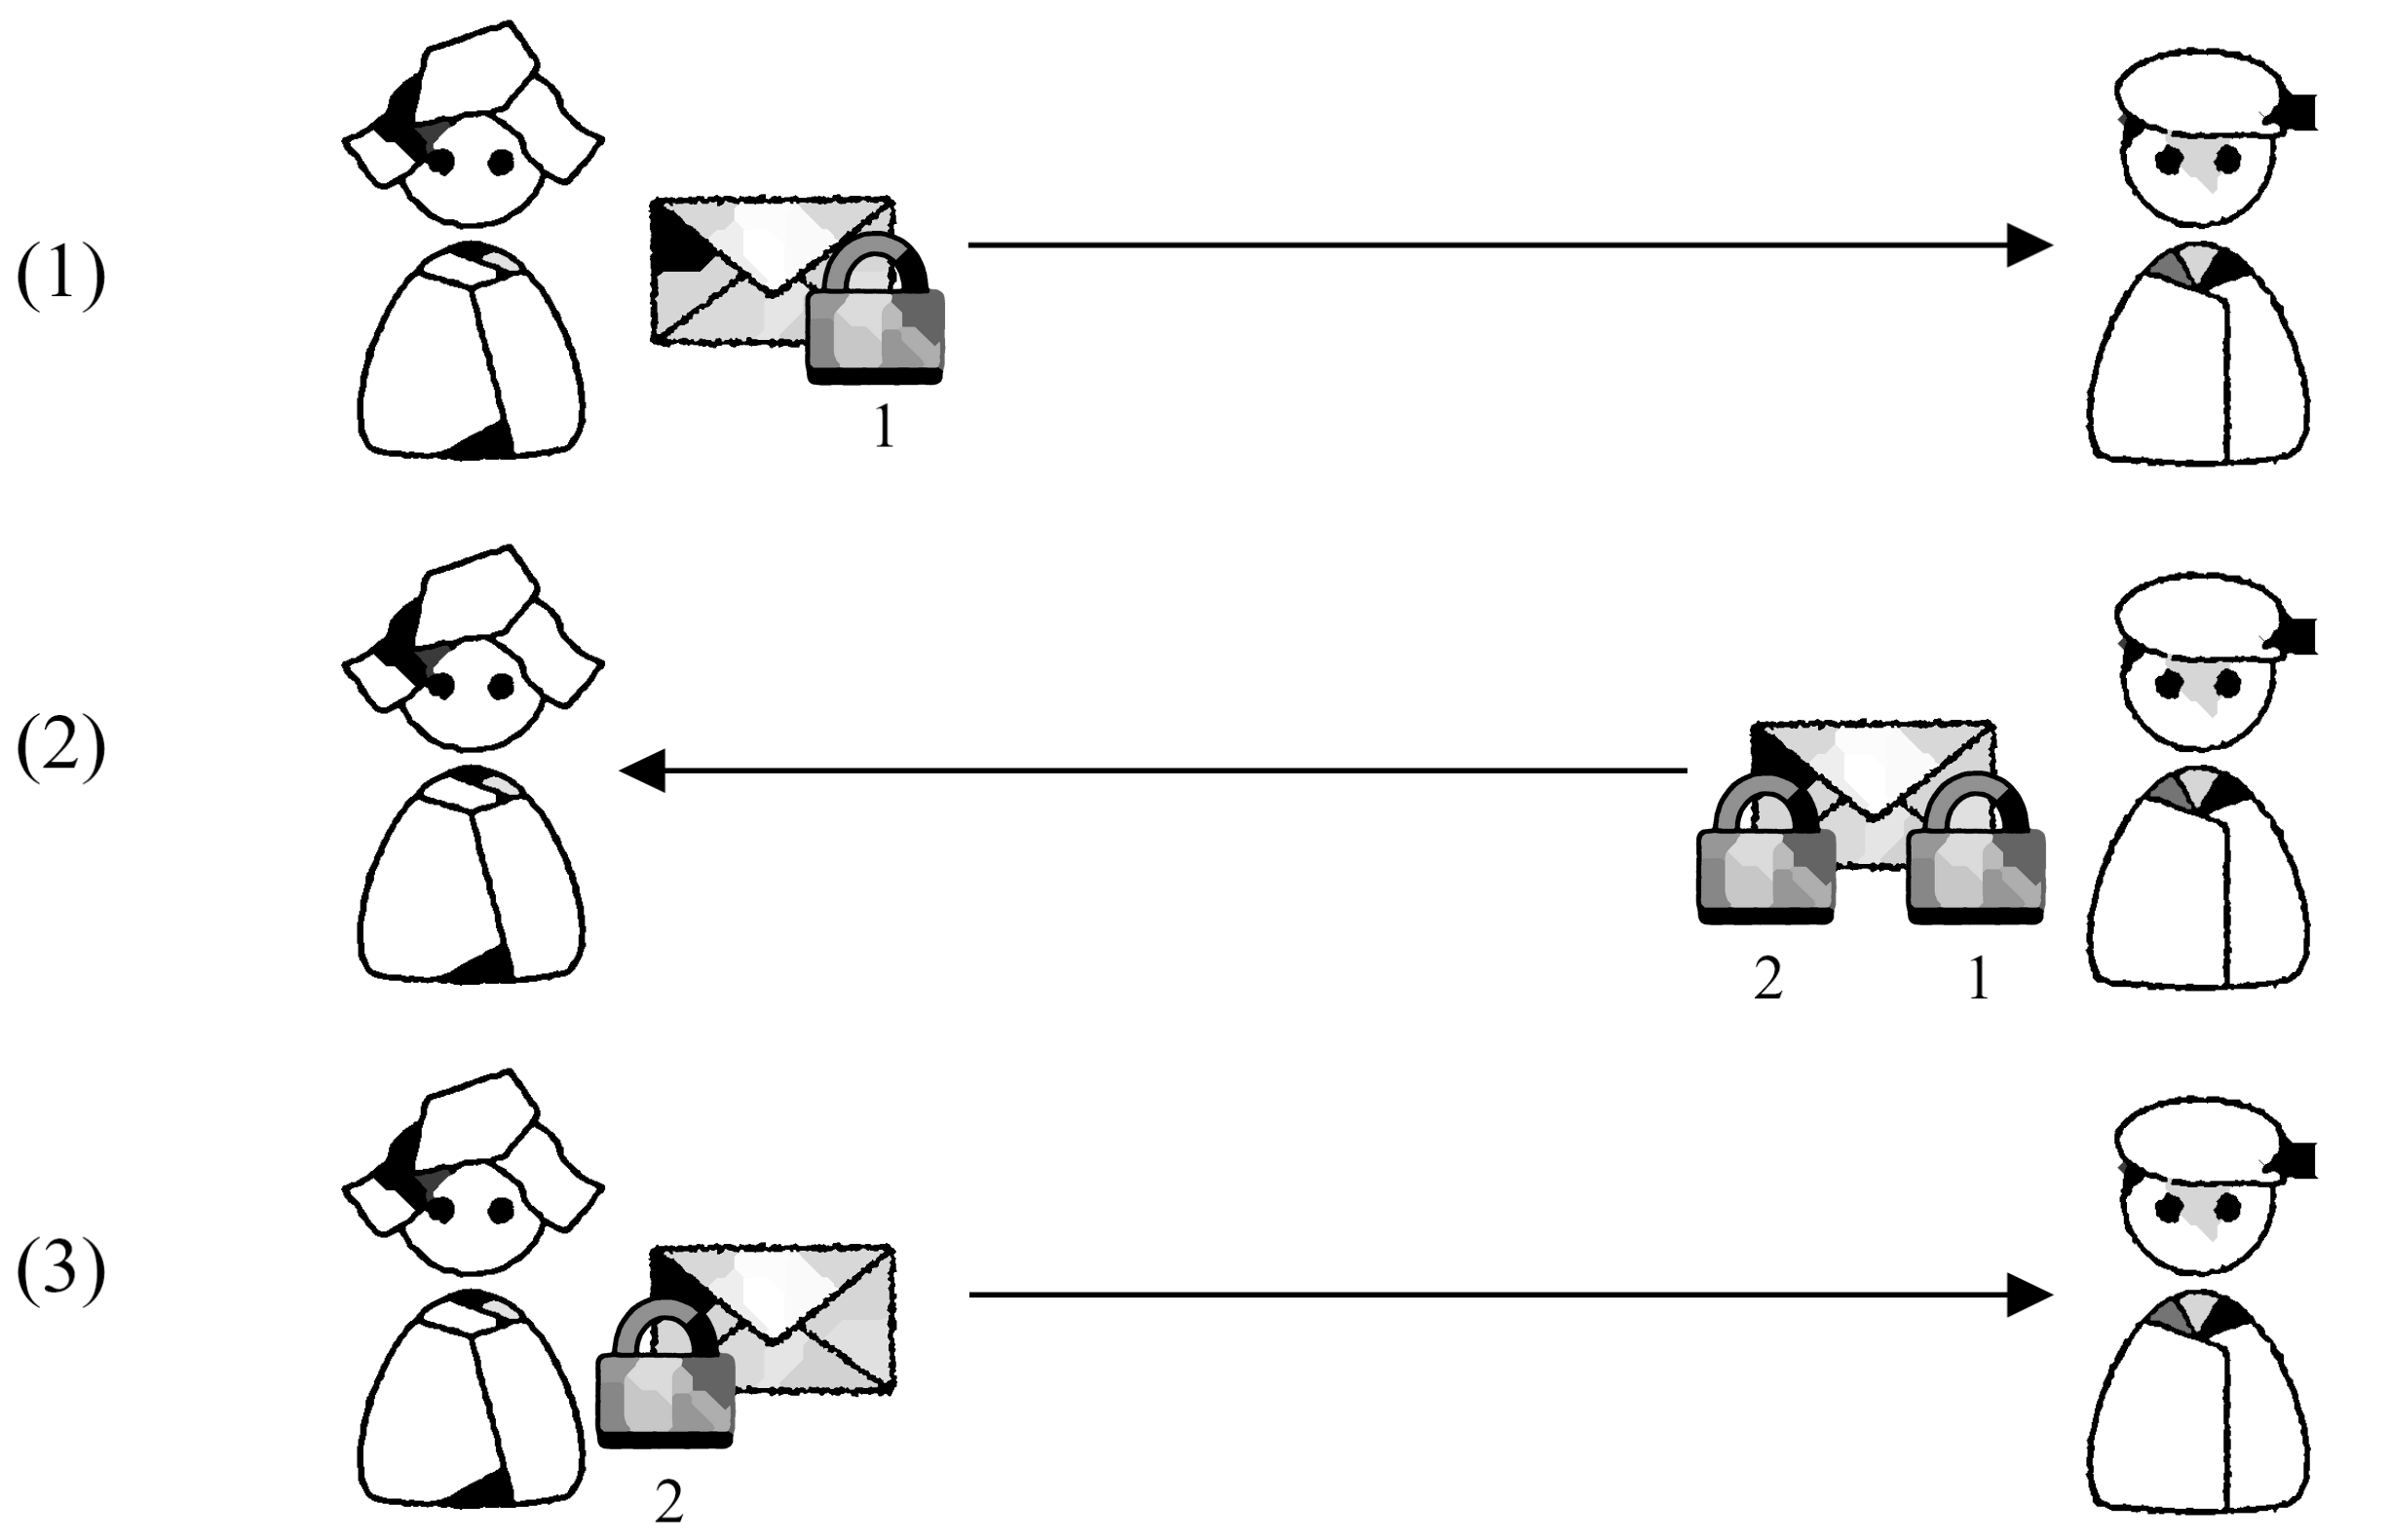
\includegraphics[width=.7\textwidth]{Sections/sec/enc/dh/pass.png}
    \caption{Alice and Bob send a secure message via alternating locks.}
    \label{fig:dh}
\end{figure}

\noindent
This is the basic idea behind the following method.

\newpage 

\begin{Def}[Diffie-Hellman Key Exchange (DHE)]
    \label{def:dh}
    The \textbf{Diffie-Hellman Key Exchange} is a method for two parties $A$ and $B$ to establish a shared secret over an insecure channel.
    The method is as follows:
    \begin{enumerate}
        \item $A$ and $B$ agree on a prime number $p$ and a generator $g$.
        \item Both $A$ and $B$ select exponents $a$ and $b$ (secret key), and computes $\alpha=g^a \text{ mod } p$ and $\beta =g^b \text{ mod } p$ respectively.
        \item $A$ and $B$ exchange $\alpha$ (alpha) and $\beta$ (beta).
        \item $A$ computes $\lambda = \beta^a \text{ mod } p= (g^b)^a \text{ mod } p$.
        \item $B$ computes $\lambda = \alpha^b \text{ mod } p= (g^a)^b \text{ mod } p$.
    \end{enumerate}
    \noindent
    Both $A$ and $B$ establish a shared secret $\lambda$ without exchanging their secret keys. \hfill \cite{goldberg_cs357}
\end{Def}

\begin{figure}[h!]
    \centering
    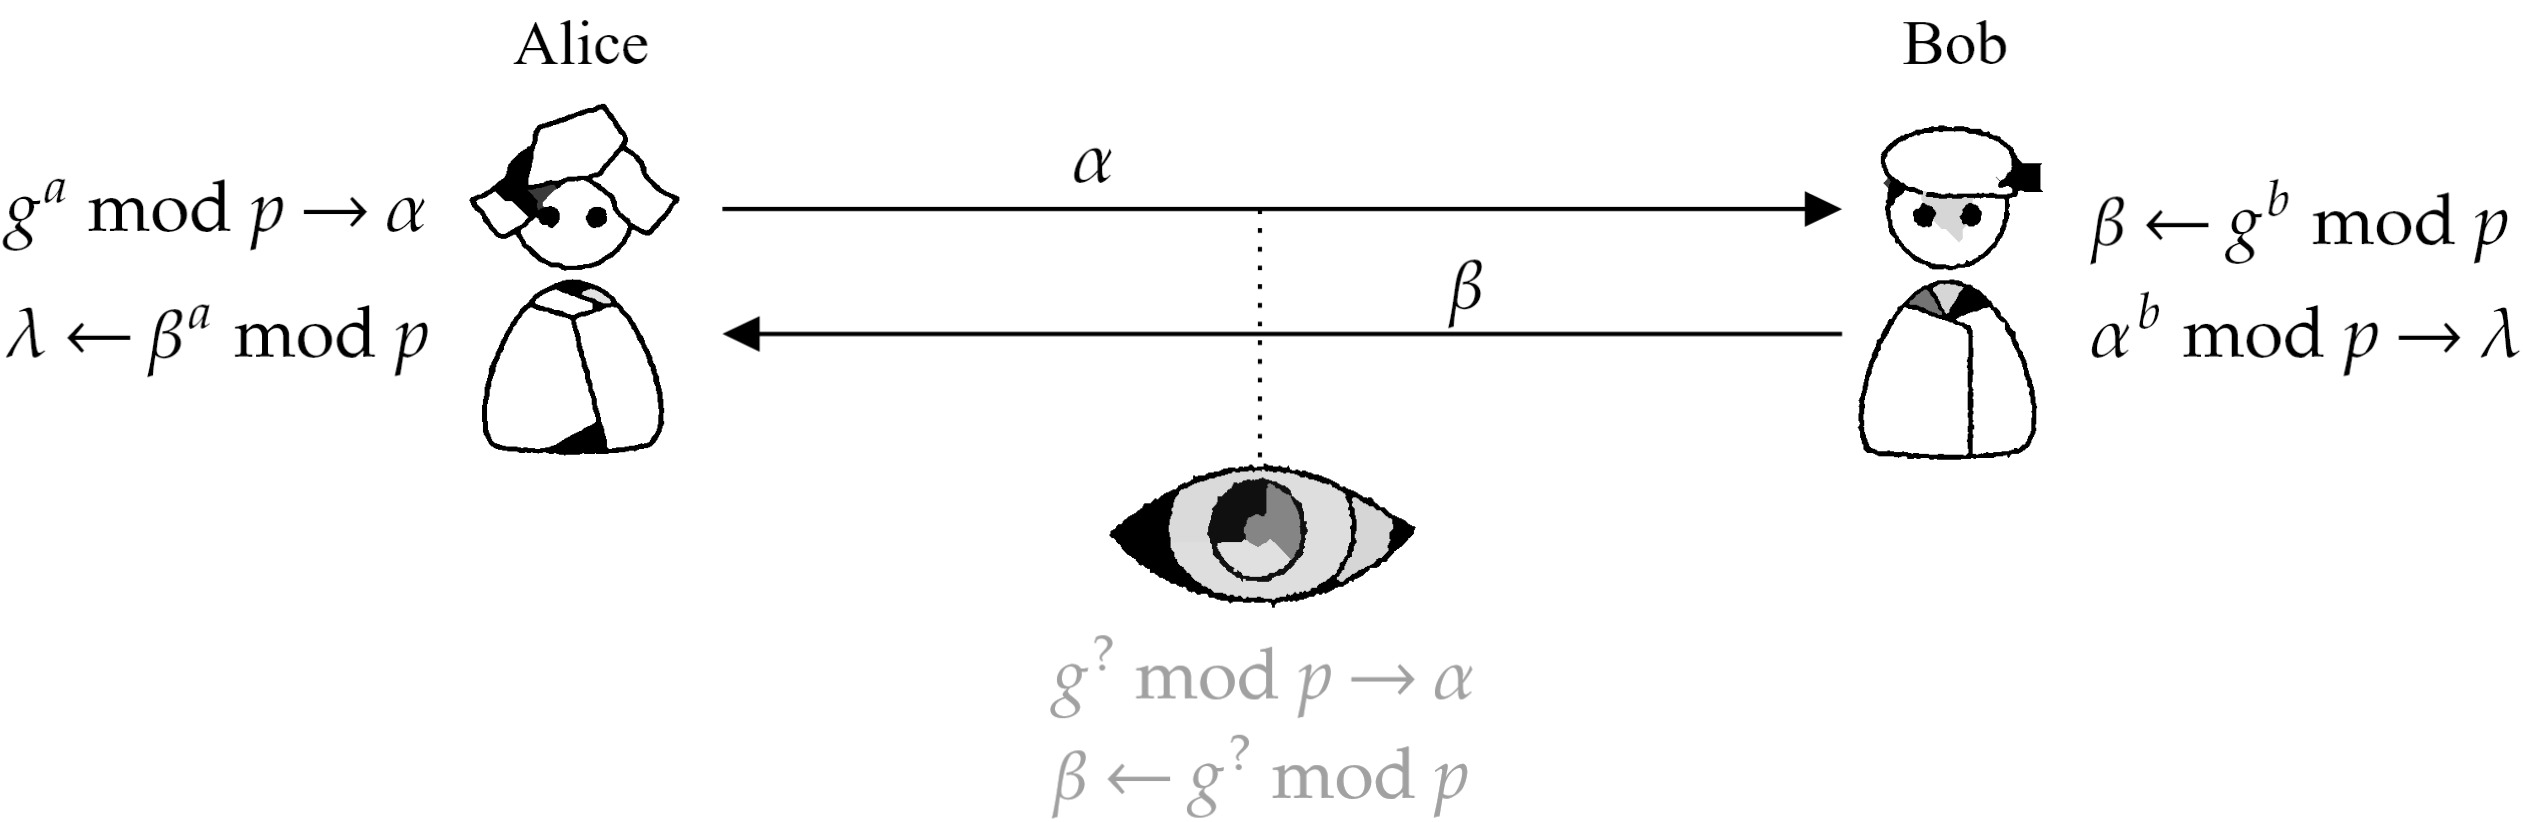
\includegraphics[width=.9\textwidth]{Sections/sec/enc/dh/dh.png}
    \caption{Diffie-Hellman Key Exchange protects against eavesdropping.}
    \label{fig:dh}
\end{figure}

\noindent
However,
\begin{figure}[h!]
    \centering
    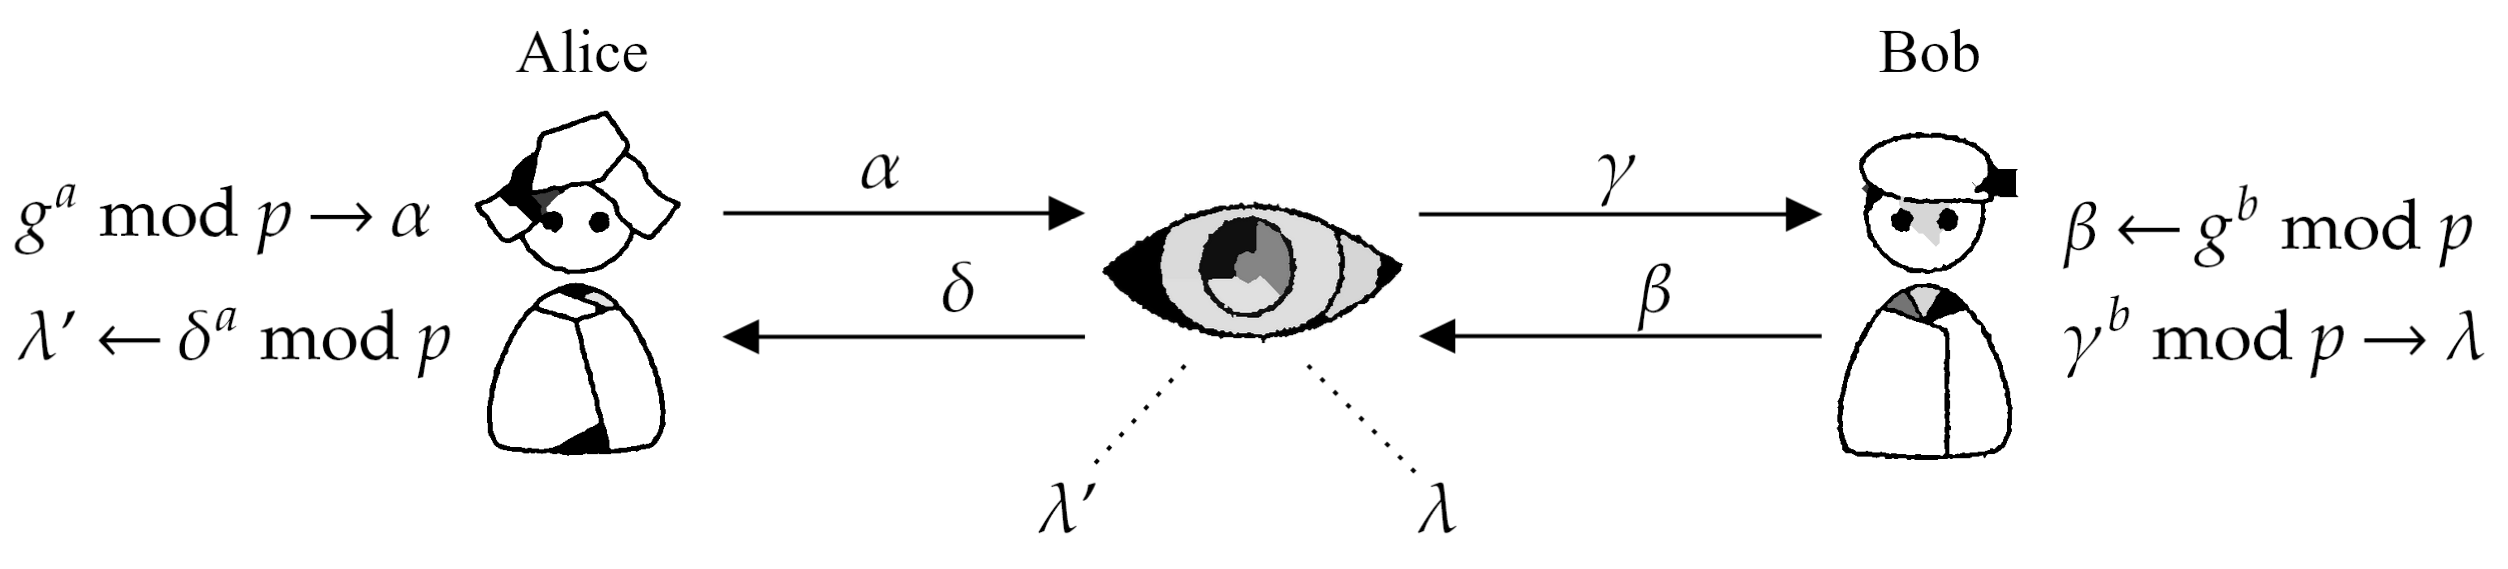
\includegraphics[width=.9\textwidth]{Sections/sec/enc/dh/mitm.png}
    \caption{Diffie-Hellman Key Exchange Attack via MITM.}
    \label{fig:dh}
\end{figure}

\noindent
If Alice and Bob were purely trying to connect on their own, there would be no way to verify that they are who they say they are.

\newpage

\noindent
Though this can be fixed by a previous topic discussed, \textbf{Public Key Infrastructure (PKI)}. If 
Alice and Bob had a certificate from a trusted third party, they could verify each other's identity.

\begin{figure}[h!]
    \centering
    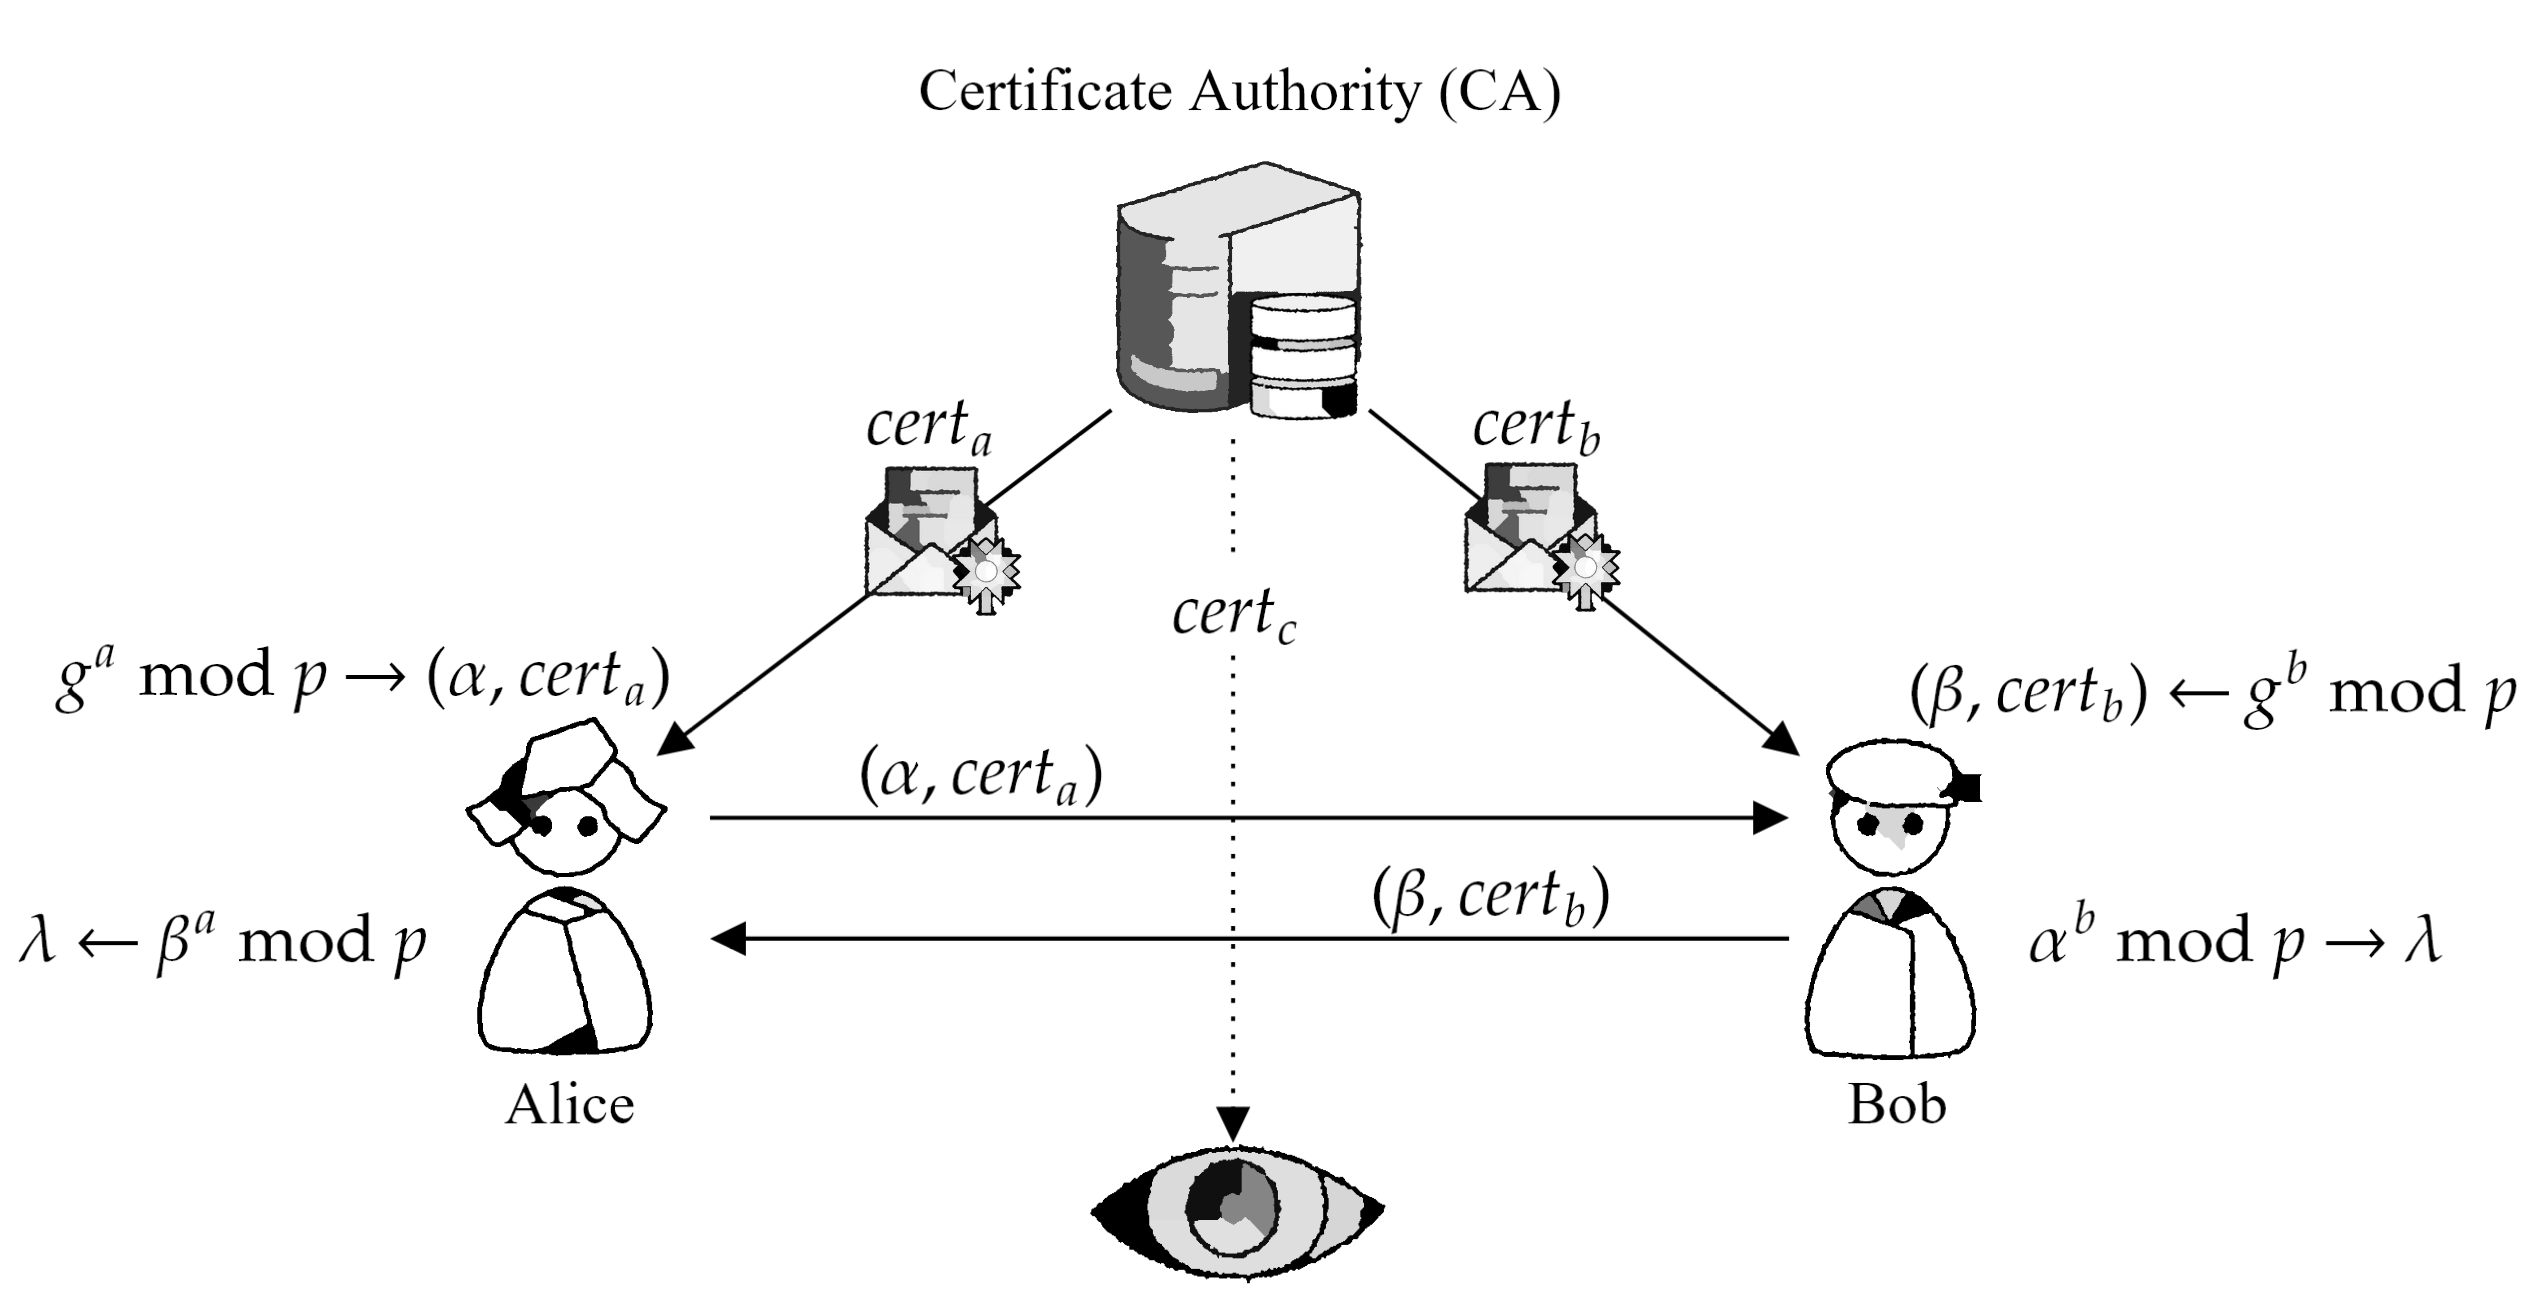
\includegraphics[width=.9\textwidth]{Sections/sec/enc/dh/pki.png}
    \caption{Diffie-Hellman Key Exchange with PKI.}
    \label{fig:dh}
\end{figure}

\noindent
Here Alice and Bob previously made a CSR (Certificate Signing Request) to a CA (Certificate Authority) to get a certificate. Here the
CA---a trusted entity that predominately come pre-baked into OSs and Web Browsers---signs Alice and Bob's certificate. This way,
Alice and Bob may verify each other's identity via signing their data and sharing a public key.

An adversary cannot forge a signature without the certificates' private keys, and cannot forge a certificate as only CA's can issue them via their own private key.
Recall certificates come with identifying information of who the certificate belongs to and the issuer.

\begin{theo}[Authenticated Diffie-Hellman Key Exchange]

    \label{theo:dh}
    The \textbf{Authenticated Diffie-Hellman Key Exchange} is a method for two parties $A$ and $B$ to establish a shared secret over an insecure channel, with the help of a trusted third party.
    Before performing the Diffie-Hellman Key Exchange (DHE), $A$ and $B$ obtain certificates from a Certificate Authority (CA) via a Certificate Signing Request (CSR).
    Once the certificates are obtained, both parties can perform DHE via signing and verifying data sent. \hfill \cite{goldberg_cs357}
\end{theo}

\begin{theo}[Post DHE Data Exchange]

    \label{theo:dh}
    After DHE is complete between parties $A$ and $B$, they may now communicate 
    via symmetric encryption. Moreover, they can use MACs to ensure data integrity, or in particular, AES in GCM providing encryption.
\end{theo}